\documentclass{standalone}
\usepackage{tikz}
\begin{document}
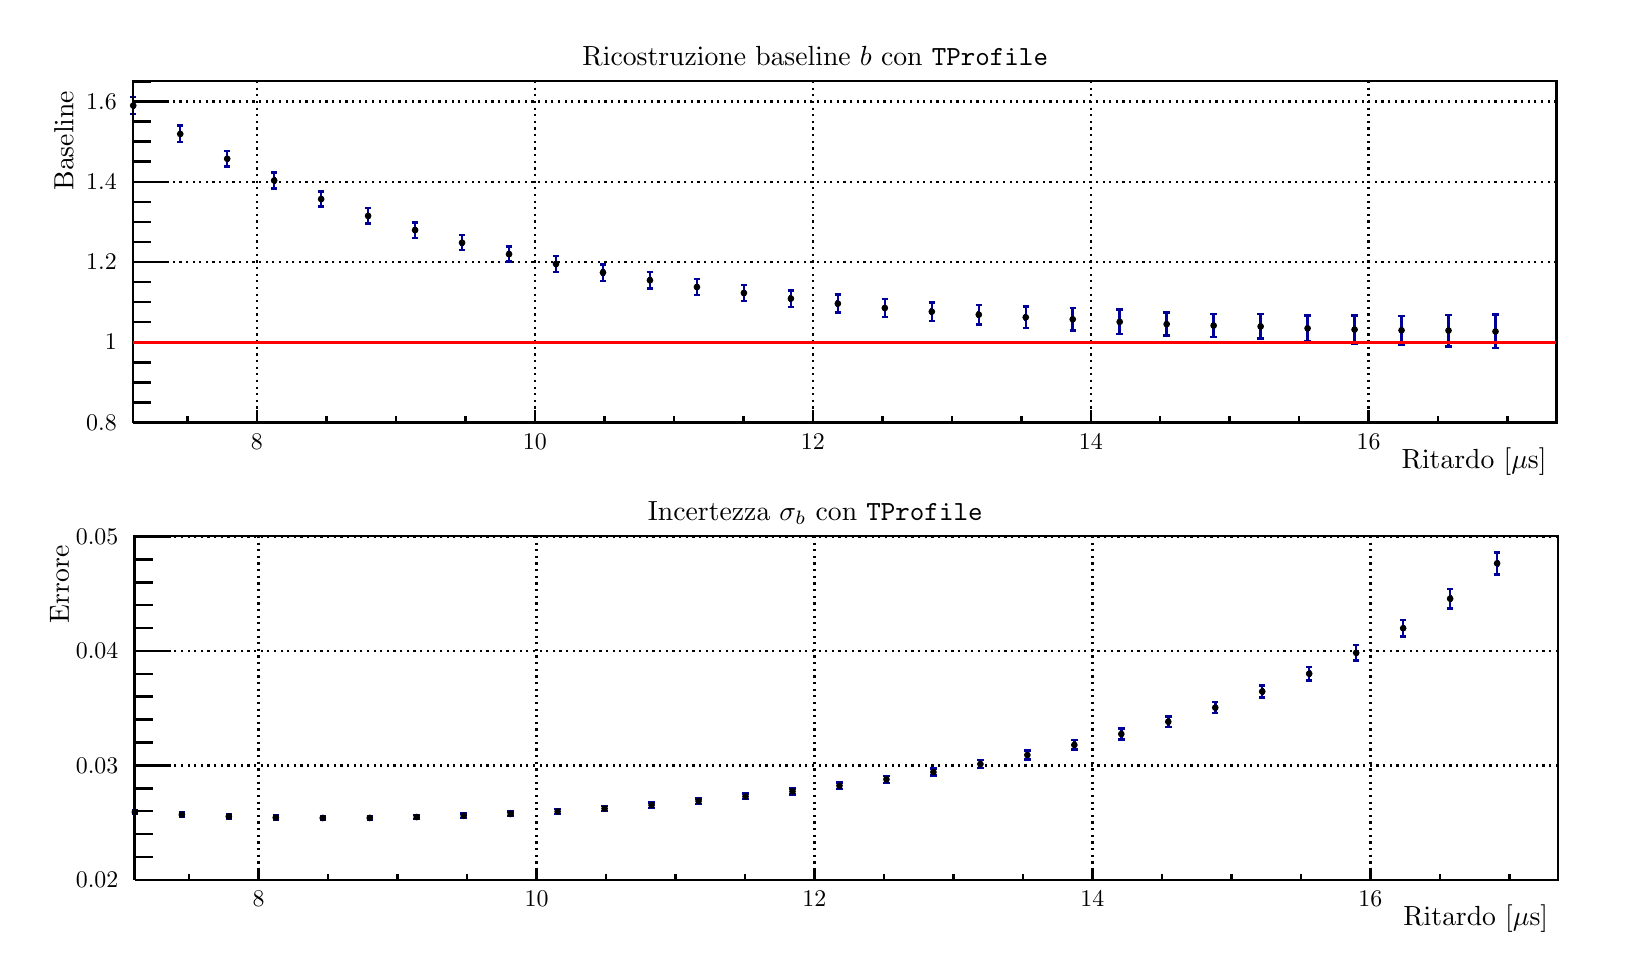
\begin{tikzpicture}
\pgfdeclareplotmark{cross} {
\pgfpathmoveto{\pgfpoint{-0.3\pgfplotmarksize}{\pgfplotmarksize}}
\pgfpathlineto{\pgfpoint{+0.3\pgfplotmarksize}{\pgfplotmarksize}}
\pgfpathlineto{\pgfpoint{+0.3\pgfplotmarksize}{0.3\pgfplotmarksize}}
\pgfpathlineto{\pgfpoint{+1\pgfplotmarksize}{0.3\pgfplotmarksize}}
\pgfpathlineto{\pgfpoint{+1\pgfplotmarksize}{-0.3\pgfplotmarksize}}
\pgfpathlineto{\pgfpoint{+0.3\pgfplotmarksize}{-0.3\pgfplotmarksize}}
\pgfpathlineto{\pgfpoint{+0.3\pgfplotmarksize}{-1.\pgfplotmarksize}}
\pgfpathlineto{\pgfpoint{-0.3\pgfplotmarksize}{-1.\pgfplotmarksize}}
\pgfpathlineto{\pgfpoint{-0.3\pgfplotmarksize}{-0.3\pgfplotmarksize}}
\pgfpathlineto{\pgfpoint{-1.\pgfplotmarksize}{-0.3\pgfplotmarksize}}
\pgfpathlineto{\pgfpoint{-1.\pgfplotmarksize}{0.3\pgfplotmarksize}}
\pgfpathlineto{\pgfpoint{-0.3\pgfplotmarksize}{0.3\pgfplotmarksize}}
\pgfpathclose
\pgfusepathqstroke
}
\pgfdeclareplotmark{cross*} {
\pgfpathmoveto{\pgfpoint{-0.3\pgfplotmarksize}{\pgfplotmarksize}}
\pgfpathlineto{\pgfpoint{+0.3\pgfplotmarksize}{\pgfplotmarksize}}
\pgfpathlineto{\pgfpoint{+0.3\pgfplotmarksize}{0.3\pgfplotmarksize}}
\pgfpathlineto{\pgfpoint{+1\pgfplotmarksize}{0.3\pgfplotmarksize}}
\pgfpathlineto{\pgfpoint{+1\pgfplotmarksize}{-0.3\pgfplotmarksize}}
\pgfpathlineto{\pgfpoint{+0.3\pgfplotmarksize}{-0.3\pgfplotmarksize}}
\pgfpathlineto{\pgfpoint{+0.3\pgfplotmarksize}{-1.\pgfplotmarksize}}
\pgfpathlineto{\pgfpoint{-0.3\pgfplotmarksize}{-1.\pgfplotmarksize}}
\pgfpathlineto{\pgfpoint{-0.3\pgfplotmarksize}{-0.3\pgfplotmarksize}}
\pgfpathlineto{\pgfpoint{-1.\pgfplotmarksize}{-0.3\pgfplotmarksize}}
\pgfpathlineto{\pgfpoint{-1.\pgfplotmarksize}{0.3\pgfplotmarksize}}
\pgfpathlineto{\pgfpoint{-0.3\pgfplotmarksize}{0.3\pgfplotmarksize}}
\pgfpathclose
\pgfusepathqfillstroke
}
\pgfdeclareplotmark{newstar} {
\pgfpathmoveto{\pgfqpoint{0pt}{\pgfplotmarksize}}
\pgfpathlineto{\pgfqpointpolar{44}{0.5\pgfplotmarksize}}
\pgfpathlineto{\pgfqpointpolar{18}{\pgfplotmarksize}}
\pgfpathlineto{\pgfqpointpolar{-20}{0.5\pgfplotmarksize}}
\pgfpathlineto{\pgfqpointpolar{-54}{\pgfplotmarksize}}
\pgfpathlineto{\pgfqpointpolar{-90}{0.5\pgfplotmarksize}}
\pgfpathlineto{\pgfqpointpolar{234}{\pgfplotmarksize}}
\pgfpathlineto{\pgfqpointpolar{198}{0.5\pgfplotmarksize}}
\pgfpathlineto{\pgfqpointpolar{162}{\pgfplotmarksize}}
\pgfpathlineto{\pgfqpointpolar{134}{0.5\pgfplotmarksize}}
\pgfpathclose
\pgfusepathqstroke
}
\pgfdeclareplotmark{newstar*} {
\pgfpathmoveto{\pgfqpoint{0pt}{\pgfplotmarksize}}
\pgfpathlineto{\pgfqpointpolar{44}{0.5\pgfplotmarksize}}
\pgfpathlineto{\pgfqpointpolar{18}{\pgfplotmarksize}}
\pgfpathlineto{\pgfqpointpolar{-20}{0.5\pgfplotmarksize}}
\pgfpathlineto{\pgfqpointpolar{-54}{\pgfplotmarksize}}
\pgfpathlineto{\pgfqpointpolar{-90}{0.5\pgfplotmarksize}}
\pgfpathlineto{\pgfqpointpolar{234}{\pgfplotmarksize}}
\pgfpathlineto{\pgfqpointpolar{198}{0.5\pgfplotmarksize}}
\pgfpathlineto{\pgfqpointpolar{162}{\pgfplotmarksize}}
\pgfpathlineto{\pgfqpointpolar{134}{0.5\pgfplotmarksize}}
\pgfpathclose
\pgfusepathqfillstroke
}
\definecolor{c}{rgb}{1,1,1};
\draw [color=c, fill=c] (0,0) rectangle (20,11.5542);
\draw [color=c, fill=c] (0.2,5.89264) rectangle (19.8,11.4387);
\draw [color=c, fill=c] (1.32924,6.54669) rectangle (19.407,10.884);
\definecolor{c}{rgb}{0,0,0};
\draw [c,line width=0.9] (1.32924,6.54669) -- (1.32924,10.884) -- (19.407,10.884) -- (19.407,6.54669) -- (1.32924,6.54669);
\definecolor{c}{rgb}{1,1,1};
\draw [color=c, fill=c] (1.32924,6.54669) rectangle (19.407,10.884);
\definecolor{c}{rgb}{0,0,0};
\draw [c,line width=0.9] (1.32924,6.54669) -- (1.32924,10.884) -- (19.407,10.884) -- (19.407,6.54669) -- (1.32924,6.54669);
\draw [c,line width=0.9] (1.32924,6.54669) -- (19.407,6.54669);
\draw [c,dash pattern=on 0.80pt off 1.60pt ,line width=0.9] (2.90505,10.884) -- (2.90505,6.54669);
\draw [c,dash pattern=on 0.80pt off 1.60pt ,line width=0.9] (6.43474,10.884) -- (6.43474,6.54669);
\draw [c,dash pattern=on 0.80pt off 1.60pt ,line width=0.9] (9.96442,10.884) -- (9.96442,6.54669);
\draw [c,dash pattern=on 0.80pt off 1.60pt ,line width=0.9] (13.4941,10.884) -- (13.4941,6.54669);
\draw [c,dash pattern=on 0.80pt off 1.60pt ,line width=0.9] (17.0238,10.884) -- (17.0238,6.54669);
\draw [c,dash pattern=on 0.80pt off 1.60pt ,line width=0.9] (2.90505,10.884) -- (2.90505,6.54669);
\draw [c,dash pattern=on 0.80pt off 1.60pt ,line width=0.9] (17.0238,10.884) -- (17.0238,6.54669);
\draw [c,line width=0.9] (1.32924,6.54669) -- (1.32924,10.884);
\draw [c,dash pattern=on 0.80pt off 1.60pt ,line width=0.9] (19.407,6.54669) -- (1.32924,6.54669);
\draw [c,dash pattern=on 0.80pt off 1.60pt ,line width=0.9] (19.407,7.56584) -- (1.32924,7.56584);
\draw [c,dash pattern=on 0.80pt off 1.60pt ,line width=0.9] (19.407,8.58499) -- (1.32924,8.58499);
\draw [c,dash pattern=on 0.80pt off 1.60pt ,line width=0.9] (19.407,9.60415) -- (1.32924,9.60415);
\draw [c,dash pattern=on 0.80pt off 1.60pt ,line width=0.9] (19.407,10.6233) -- (1.32924,10.6233);
\draw [c,dash pattern=on 0.80pt off 1.60pt ,line width=0.9] (19.407,10.6233) -- (1.32924,10.6233);
\definecolor{c}{rgb}{0,0,0.6};
\draw [c,line width=0.9] (1.33376,10.4656) -- (1.33376,10.5715);
\draw [c,line width=0.9] (1.33376,10.5715) -- (1.33376,10.6775);
\draw [c,line width=0.9] (1.32924,10.5715) -- (1.33376,10.5715);
\draw [c,line width=0.9] (1.33376,10.5715) -- (1.33828,10.5715);
\draw [c,line width=0.9] (1.29286,10.4656) -- (1.37466,10.4656);
\draw [c,line width=0.9] (1.29286,10.6775) -- (1.37466,10.6775);
\draw [c,line width=0.9] (1.32924,10.5306) -- (1.32924,10.6124);
\draw [c,line width=0.9] (1.33828,10.5306) -- (1.33828,10.6124);
\definecolor{c}{rgb}{0,0,0};
\foreach \P in {(1.33376,10.5715)}{\draw[mark options={color=c,fill=c},mark size=2.402402pt,mark=*,mark size=1pt] plot coordinates {\P};}
\definecolor{c}{rgb}{0,0,0.6};
\draw [c,line width=0.9] (1.93033,10.1063) -- (1.93033,10.2114);
\draw [c,line width=0.9] (1.93033,10.2114) -- (1.93033,10.3165);
\draw [c,line width=0.9] (1.92581,10.2114) -- (1.93033,10.2114);
\draw [c,line width=0.9] (1.93033,10.2114) -- (1.93485,10.2114);
\draw [c,line width=0.9] (1.88943,10.1063) -- (1.97123,10.1063);
\draw [c,line width=0.9] (1.88943,10.3165) -- (1.97123,10.3165);
\draw [c,line width=0.9] (1.92581,10.1705) -- (1.92581,10.2523);
\draw [c,line width=0.9] (1.93485,10.1705) -- (1.93485,10.2523);
\definecolor{c}{rgb}{0,0,0};
\foreach \P in {(1.93033,10.2114)}{\draw[mark options={color=c,fill=c},mark size=2.402402pt,mark=*,mark size=1pt] plot coordinates {\P};}
\definecolor{c}{rgb}{0,0,0.6};
\draw [c,line width=0.9] (2.52689,9.79651) -- (2.52689,9.89609);
\draw [c,line width=0.9] (2.52689,9.89609) -- (2.52689,9.99566);
\draw [c,line width=0.9] (2.52237,9.89609) -- (2.52689,9.89609);
\draw [c,line width=0.9] (2.52689,9.89609) -- (2.53141,9.89609);
\draw [c,line width=0.9] (2.48599,9.79651) -- (2.56779,9.79651);
\draw [c,line width=0.9] (2.48599,9.99566) -- (2.56779,9.99566);
\draw [c,line width=0.9] (2.52237,9.85519) -- (2.52237,9.93699);
\draw [c,line width=0.9] (2.53141,9.85519) -- (2.53141,9.93699);
\definecolor{c}{rgb}{0,0,0};
\foreach \P in {(2.52689,9.89609)}{\draw[mark options={color=c,fill=c},mark size=2.402402pt,mark=*,mark size=1pt] plot coordinates {\P};}
\definecolor{c}{rgb}{0,0,0.6};
\draw [c,line width=0.9] (3.12346,9.51936) -- (3.12346,9.62001);
\draw [c,line width=0.9] (3.12346,9.62001) -- (3.12346,9.72065);
\draw [c,line width=0.9] (3.11894,9.62001) -- (3.12346,9.62001);
\draw [c,line width=0.9] (3.12346,9.62001) -- (3.12798,9.62001);
\draw [c,line width=0.9] (3.08256,9.51936) -- (3.16436,9.51936);
\draw [c,line width=0.9] (3.08256,9.72065) -- (3.16436,9.72065);
\draw [c,line width=0.9] (3.11894,9.57911) -- (3.11894,9.66091);
\draw [c,line width=0.9] (3.12798,9.57911) -- (3.12798,9.66091);
\definecolor{c}{rgb}{0,0,0};
\foreach \P in {(3.12346,9.62001)}{\draw[mark options={color=c,fill=c},mark size=2.402402pt,mark=*,mark size=1pt] plot coordinates {\P};}
\definecolor{c}{rgb}{0,0,0.6};
\draw [c,line width=0.9] (3.72002,9.28788) -- (3.72002,9.3847);
\draw [c,line width=0.9] (3.72002,9.3847) -- (3.72002,9.48151);
\draw [c,line width=0.9] (3.7155,9.3847) -- (3.72002,9.3847);
\draw [c,line width=0.9] (3.72002,9.3847) -- (3.72454,9.3847);
\draw [c,line width=0.9] (3.67912,9.28788) -- (3.76092,9.28788);
\draw [c,line width=0.9] (3.67912,9.48151) -- (3.76092,9.48151);
\draw [c,line width=0.9] (3.7155,9.3438) -- (3.7155,9.4256);
\draw [c,line width=0.9] (3.72454,9.3438) -- (3.72454,9.4256);
\definecolor{c}{rgb}{0,0,0};
\foreach \P in {(3.72002,9.3847)}{\draw[mark options={color=c,fill=c},mark size=2.402402pt,mark=*,mark size=1pt] plot coordinates {\P};}
\definecolor{c}{rgb}{0,0,0.6};
\draw [c,line width=0.9] (4.31659,9.07182) -- (4.31659,9.1703);
\draw [c,line width=0.9] (4.31659,9.1703) -- (4.31659,9.26877);
\draw [c,line width=0.9] (4.31207,9.1703) -- (4.31659,9.1703);
\draw [c,line width=0.9] (4.31659,9.1703) -- (4.3211,9.1703);
\draw [c,line width=0.9] (4.27569,9.07182) -- (4.35748,9.07182);
\draw [c,line width=0.9] (4.27569,9.26877) -- (4.35748,9.26877);
\draw [c,line width=0.9] (4.31207,9.1294) -- (4.31207,9.2112);
\draw [c,line width=0.9] (4.3211,9.1294) -- (4.3211,9.2112);
\definecolor{c}{rgb}{0,0,0};
\foreach \P in {(4.31659,9.1703)}{\draw[mark options={color=c,fill=c},mark size=2.402402pt,mark=*,mark size=1pt] plot coordinates {\P};}
\definecolor{c}{rgb}{0,0,0.6};
\draw [c,line width=0.9] (4.91315,8.89318) -- (4.91315,8.99032);
\draw [c,line width=0.9] (4.91315,8.99032) -- (4.91315,9.08746);
\draw [c,line width=0.9] (4.90863,8.99032) -- (4.91315,8.99032);
\draw [c,line width=0.9] (4.91315,8.99032) -- (4.91767,8.99032);
\draw [c,line width=0.9] (4.87225,8.89318) -- (4.95405,8.89318);
\draw [c,line width=0.9] (4.87225,9.08746) -- (4.95405,9.08746);
\draw [c,line width=0.9] (4.90863,8.94942) -- (4.90863,9.03122);
\draw [c,line width=0.9] (4.91767,8.94942) -- (4.91767,9.03122);
\definecolor{c}{rgb}{0,0,0};
\foreach \P in {(4.91315,8.99032)}{\draw[mark options={color=c,fill=c},mark size=2.402402pt,mark=*,mark size=1pt] plot coordinates {\P};}
\definecolor{c}{rgb}{0,0,0.6};
\draw [c,line width=0.9] (5.50971,8.73507) -- (5.50971,8.82999);
\draw [c,line width=0.9] (5.50971,8.82999) -- (5.50971,8.92491);
\draw [c,line width=0.9] (5.50519,8.82999) -- (5.50971,8.82999);
\draw [c,line width=0.9] (5.50971,8.82999) -- (5.51423,8.82999);
\draw [c,line width=0.9] (5.46881,8.73507) -- (5.55061,8.73507);
\draw [c,line width=0.9] (5.46881,8.92491) -- (5.55061,8.92491);
\draw [c,line width=0.9] (5.50519,8.78909) -- (5.50519,8.87089);
\draw [c,line width=0.9] (5.51423,8.78909) -- (5.51423,8.87089);
\definecolor{c}{rgb}{0,0,0};
\foreach \P in {(5.50971,8.82999)}{\draw[mark options={color=c,fill=c},mark size=2.402402pt,mark=*,mark size=1pt] plot coordinates {\P};}
\definecolor{c}{rgb}{0,0,0.6};
\draw [c,line width=0.9] (6.10628,8.58875) -- (6.10628,8.68491);
\draw [c,line width=0.9] (6.10628,8.68491) -- (6.10628,8.78108);
\draw [c,line width=0.9] (6.10176,8.68491) -- (6.10628,8.68491);
\draw [c,line width=0.9] (6.10628,8.68491) -- (6.1108,8.68491);
\draw [c,line width=0.9] (6.06538,8.58875) -- (6.14718,8.58875);
\draw [c,line width=0.9] (6.06538,8.78108) -- (6.14718,8.78108);
\draw [c,line width=0.9] (6.10176,8.64401) -- (6.10176,8.72581);
\draw [c,line width=0.9] (6.1108,8.64401) -- (6.1108,8.72581);
\definecolor{c}{rgb}{0,0,0};
\foreach \P in {(6.10628,8.68491)}{\draw[mark options={color=c,fill=c},mark size=2.402402pt,mark=*,mark size=1pt] plot coordinates {\P};}
\definecolor{c}{rgb}{0,0,0.6};
\draw [c,line width=0.9] (6.70284,8.46081) -- (6.70284,8.5611);
\draw [c,line width=0.9] (6.70284,8.5611) -- (6.70284,8.66138);
\draw [c,line width=0.9] (6.69832,8.5611) -- (6.70284,8.5611);
\draw [c,line width=0.9] (6.70284,8.5611) -- (6.70736,8.5611);
\draw [c,line width=0.9] (6.66194,8.46081) -- (6.74374,8.46081);
\draw [c,line width=0.9] (6.66194,8.66138) -- (6.74374,8.66138);
\draw [c,line width=0.9] (6.69832,8.5202) -- (6.69832,8.602);
\draw [c,line width=0.9] (6.70736,8.5202) -- (6.70736,8.602);
\definecolor{c}{rgb}{0,0,0};
\foreach \P in {(6.70284,8.5611)}{\draw[mark options={color=c,fill=c},mark size=2.402402pt,mark=*,mark size=1pt] plot coordinates {\P};}
\definecolor{c}{rgb}{0,0,0.6};
\draw [c,line width=0.9] (7.29941,8.34684) -- (7.29941,8.45159);
\draw [c,line width=0.9] (7.29941,8.45159) -- (7.29941,8.55635);
\draw [c,line width=0.9] (7.29489,8.45159) -- (7.29941,8.45159);
\draw [c,line width=0.9] (7.29941,8.45159) -- (7.30393,8.45159);
\draw [c,line width=0.9] (7.25851,8.34684) -- (7.34031,8.34684);
\draw [c,line width=0.9] (7.25851,8.55635) -- (7.34031,8.55635);
\draw [c,line width=0.9] (7.29489,8.41069) -- (7.29489,8.49249);
\draw [c,line width=0.9] (7.30393,8.41069) -- (7.30393,8.49249);
\definecolor{c}{rgb}{0,0,0};
\foreach \P in {(7.29941,8.45159)}{\draw[mark options={color=c,fill=c},mark size=2.402402pt,mark=*,mark size=1pt] plot coordinates {\P};}
\definecolor{c}{rgb}{0,0,0.6};
\draw [c,line width=0.9] (7.89597,8.24775) -- (7.89597,8.35308);
\draw [c,line width=0.9] (7.89597,8.35308) -- (7.89597,8.4584);
\draw [c,line width=0.9] (7.89145,8.35308) -- (7.89597,8.35308);
\draw [c,line width=0.9] (7.89597,8.35308) -- (7.90049,8.35308);
\draw [c,line width=0.9] (7.85507,8.24775) -- (7.93687,8.24775);
\draw [c,line width=0.9] (7.85507,8.4584) -- (7.93687,8.4584);
\draw [c,line width=0.9] (7.89145,8.31218) -- (7.89145,8.39398);
\draw [c,line width=0.9] (7.90049,8.31218) -- (7.90049,8.39398);
\definecolor{c}{rgb}{0,0,0};
\foreach \P in {(7.89597,8.35308)}{\draw[mark options={color=c,fill=c},mark size=2.402402pt,mark=*,mark size=1pt] plot coordinates {\P};}
\definecolor{c}{rgb}{0,0,0.6};
\draw [c,line width=0.9] (8.49254,8.16462) -- (8.49254,8.26746);
\draw [c,line width=0.9] (8.49254,8.26746) -- (8.49254,8.37031);
\draw [c,line width=0.9] (8.48802,8.26746) -- (8.49254,8.26746);
\draw [c,line width=0.9] (8.49254,8.26746) -- (8.49706,8.26746);
\draw [c,line width=0.9] (8.45164,8.16462) -- (8.53344,8.16462);
\draw [c,line width=0.9] (8.45164,8.37031) -- (8.53344,8.37031);
\draw [c,line width=0.9] (8.48802,8.22656) -- (8.48802,8.30836);
\draw [c,line width=0.9] (8.49706,8.22656) -- (8.49706,8.30836);
\definecolor{c}{rgb}{0,0,0};
\foreach \P in {(8.49254,8.26746)}{\draw[mark options={color=c,fill=c},mark size=2.402402pt,mark=*,mark size=1pt] plot coordinates {\P};}
\definecolor{c}{rgb}{0,0,0.6};
\draw [c,line width=0.9] (9.0891,8.09194) -- (9.0891,8.1921);
\draw [c,line width=0.9] (9.0891,8.1921) -- (9.0891,8.29225);
\draw [c,line width=0.9] (9.08458,8.1921) -- (9.0891,8.1921);
\draw [c,line width=0.9] (9.0891,8.1921) -- (9.09362,8.1921);
\draw [c,line width=0.9] (9.0482,8.09194) -- (9.13,8.09194);
\draw [c,line width=0.9] (9.0482,8.29225) -- (9.13,8.29225);
\draw [c,line width=0.9] (9.08458,8.1512) -- (9.08458,8.233);
\draw [c,line width=0.9] (9.09362,8.1512) -- (9.09362,8.233);
\definecolor{c}{rgb}{0,0,0};
\foreach \P in {(9.0891,8.1921)}{\draw[mark options={color=c,fill=c},mark size=2.402402pt,mark=*,mark size=1pt] plot coordinates {\P};}
\definecolor{c}{rgb}{0,0,0.6};
\draw [c,line width=0.9] (9.68567,8.01611) -- (9.68567,8.12043);
\draw [c,line width=0.9] (9.68567,8.12043) -- (9.68567,8.22476);
\draw [c,line width=0.9] (9.68115,8.12043) -- (9.68567,8.12043);
\draw [c,line width=0.9] (9.68567,8.12043) -- (9.69018,8.12043);
\draw [c,line width=0.9] (9.64476,8.01611) -- (9.72656,8.01611);
\draw [c,line width=0.9] (9.64476,8.22476) -- (9.72656,8.22476);
\draw [c,line width=0.9] (9.68115,8.07953) -- (9.68115,8.16133);
\draw [c,line width=0.9] (9.69018,8.07953) -- (9.69018,8.16133);
\definecolor{c}{rgb}{0,0,0};
\foreach \P in {(9.68567,8.12043)}{\draw[mark options={color=c,fill=c},mark size=2.402402pt,mark=*,mark size=1pt] plot coordinates {\P};}
\definecolor{c}{rgb}{0,0,0.6};
\draw [c,line width=0.9] (10.2822,7.94233) -- (10.2822,8.05652);
\draw [c,line width=0.9] (10.2822,8.05652) -- (10.2822,8.17071);
\draw [c,line width=0.9] (10.2777,8.05652) -- (10.2822,8.05652);
\draw [c,line width=0.9] (10.2822,8.05652) -- (10.2867,8.05652);
\draw [c,line width=0.9] (10.2413,7.94233) -- (10.3231,7.94233);
\draw [c,line width=0.9] (10.2413,8.17071) -- (10.3231,8.17071);
\draw [c,line width=0.9] (10.2777,8.01562) -- (10.2777,8.09742);
\draw [c,line width=0.9] (10.2867,8.01562) -- (10.2867,8.09742);
\definecolor{c}{rgb}{0,0,0};
\foreach \P in {(10.2822,8.05652)}{\draw[mark options={color=c,fill=c},mark size=2.402402pt,mark=*,mark size=1pt] plot coordinates {\P};}
\definecolor{c}{rgb}{0,0,0.6};
\draw [c,line width=0.9] (10.8788,7.88482) -- (10.8788,8.00139);
\draw [c,line width=0.9] (10.8788,8.00139) -- (10.8788,8.11795);
\draw [c,line width=0.9] (10.8743,8.00139) -- (10.8788,8.00139);
\draw [c,line width=0.9] (10.8788,8.00139) -- (10.8833,8.00139);
\draw [c,line width=0.9] (10.8379,7.88482) -- (10.9197,7.88482);
\draw [c,line width=0.9] (10.8379,8.11795) -- (10.9197,8.11795);
\draw [c,line width=0.9] (10.8743,7.96049) -- (10.8743,8.04229);
\draw [c,line width=0.9] (10.8833,7.96049) -- (10.8833,8.04229);
\definecolor{c}{rgb}{0,0,0};
\foreach \P in {(10.8788,8.00139)}{\draw[mark options={color=c,fill=c},mark size=2.402402pt,mark=*,mark size=1pt] plot coordinates {\P};}
\definecolor{c}{rgb}{0,0,0.6};
\draw [c,line width=0.9] (11.4754,7.83742) -- (11.4754,7.95421);
\draw [c,line width=0.9] (11.4754,7.95421) -- (11.4754,8.071);
\draw [c,line width=0.9] (11.4708,7.95421) -- (11.4754,7.95421);
\draw [c,line width=0.9] (11.4754,7.95421) -- (11.4799,7.95421);
\draw [c,line width=0.9] (11.4345,7.83742) -- (11.5163,7.83742);
\draw [c,line width=0.9] (11.4345,8.071) -- (11.5163,8.071);
\draw [c,line width=0.9] (11.4708,7.91331) -- (11.4708,7.99511);
\draw [c,line width=0.9] (11.4799,7.91331) -- (11.4799,7.99511);
\definecolor{c}{rgb}{0,0,0};
\foreach \P in {(11.4754,7.95421)}{\draw[mark options={color=c,fill=c},mark size=2.402402pt,mark=*,mark size=1pt] plot coordinates {\P};}
\definecolor{c}{rgb}{0,0,0.6};
\draw [c,line width=0.9] (12.0719,7.79165) -- (12.0719,7.91609);
\draw [c,line width=0.9] (12.0719,7.91609) -- (12.0719,8.04054);
\draw [c,line width=0.9] (12.0674,7.91609) -- (12.0719,7.91609);
\draw [c,line width=0.9] (12.0719,7.91609) -- (12.0764,7.91609);
\draw [c,line width=0.9] (12.031,7.79165) -- (12.1128,7.79165);
\draw [c,line width=0.9] (12.031,8.04054) -- (12.1128,8.04054);
\draw [c,line width=0.9] (12.0674,7.8752) -- (12.0674,7.95699);
\draw [c,line width=0.9] (12.0764,7.8752) -- (12.0764,7.95699);
\definecolor{c}{rgb}{0,0,0};
\foreach \P in {(12.0719,7.91609)}{\draw[mark options={color=c,fill=c},mark size=2.402402pt,mark=*,mark size=1pt] plot coordinates {\P};}
\definecolor{c}{rgb}{0,0,0.6};
\draw [c,line width=0.9] (12.6685,7.74867) -- (12.6685,7.88299);
\draw [c,line width=0.9] (12.6685,7.88299) -- (12.6685,8.01731);
\draw [c,line width=0.9] (12.664,7.88299) -- (12.6685,7.88299);
\draw [c,line width=0.9] (12.6685,7.88299) -- (12.673,7.88299);
\draw [c,line width=0.9] (12.6276,7.74867) -- (12.7094,7.74867);
\draw [c,line width=0.9] (12.6276,8.01731) -- (12.7094,8.01731);
\draw [c,line width=0.9] (12.664,7.84209) -- (12.664,7.92389);
\draw [c,line width=0.9] (12.673,7.84209) -- (12.673,7.92389);
\definecolor{c}{rgb}{0,0,0};
\foreach \P in {(12.6685,7.88299)}{\draw[mark options={color=c,fill=c},mark size=2.402402pt,mark=*,mark size=1pt] plot coordinates {\P};}
\definecolor{c}{rgb}{0,0,0.6};
\draw [c,line width=0.9] (13.2651,7.71419) -- (13.2651,7.8575);
\draw [c,line width=0.9] (13.2651,7.8575) -- (13.2651,8.00081);
\draw [c,line width=0.9] (13.2605,7.8575) -- (13.2651,7.8575);
\draw [c,line width=0.9] (13.2651,7.8575) -- (13.2696,7.8575);
\draw [c,line width=0.9] (13.2242,7.71419) -- (13.306,7.71419);
\draw [c,line width=0.9] (13.2242,8.00081) -- (13.306,8.00081);
\draw [c,line width=0.9] (13.2605,7.8166) -- (13.2605,7.8984);
\draw [c,line width=0.9] (13.2696,7.8166) -- (13.2696,7.8984);
\definecolor{c}{rgb}{0,0,0};
\foreach \P in {(13.2651,7.8575)}{\draw[mark options={color=c,fill=c},mark size=2.402402pt,mark=*,mark size=1pt] plot coordinates {\P};}
\definecolor{c}{rgb}{0,0,0.6};
\draw [c,line width=0.9] (13.8616,7.66869) -- (13.8616,7.82489);
\draw [c,line width=0.9] (13.8616,7.82489) -- (13.8616,7.98109);
\draw [c,line width=0.9] (13.8571,7.82489) -- (13.8616,7.82489);
\draw [c,line width=0.9] (13.8616,7.82489) -- (13.8661,7.82489);
\draw [c,line width=0.9] (13.8207,7.66869) -- (13.9025,7.66869);
\draw [c,line width=0.9] (13.8207,7.98109) -- (13.9025,7.98109);
\draw [c,line width=0.9] (13.8571,7.78399) -- (13.8571,7.86579);
\draw [c,line width=0.9] (13.8661,7.78399) -- (13.8661,7.86579);
\definecolor{c}{rgb}{0,0,0};
\foreach \P in {(13.8616,7.82489)}{\draw[mark options={color=c,fill=c},mark size=2.402402pt,mark=*,mark size=1pt] plot coordinates {\P};}
\definecolor{c}{rgb}{0,0,0.6};
\draw [c,line width=0.9] (14.4582,7.64889) -- (14.4582,7.79626);
\draw [c,line width=0.9] (14.4582,7.79626) -- (14.4582,7.94362);
\draw [c,line width=0.9] (14.4537,7.79626) -- (14.4582,7.79626);
\draw [c,line width=0.9] (14.4582,7.79626) -- (14.4627,7.79626);
\draw [c,line width=0.9] (14.4173,7.64889) -- (14.4991,7.64889);
\draw [c,line width=0.9] (14.4173,7.94362) -- (14.4991,7.94362);
\draw [c,line width=0.9] (14.4537,7.75536) -- (14.4537,7.83716);
\draw [c,line width=0.9] (14.4627,7.75536) -- (14.4627,7.83716);
\definecolor{c}{rgb}{0,0,0};
\foreach \P in {(14.4582,7.79626)}{\draw[mark options={color=c,fill=c},mark size=2.402402pt,mark=*,mark size=1pt] plot coordinates {\P};}
\definecolor{c}{rgb}{0,0,0.6};
\draw [c,line width=0.9] (15.0547,7.63139) -- (15.0547,7.77814);
\draw [c,line width=0.9] (15.0547,7.77814) -- (15.0547,7.92488);
\draw [c,line width=0.9] (15.0502,7.77814) -- (15.0547,7.77814);
\draw [c,line width=0.9] (15.0547,7.77814) -- (15.0593,7.77814);
\draw [c,line width=0.9] (15.0138,7.63139) -- (15.0956,7.63139);
\draw [c,line width=0.9] (15.0138,7.92488) -- (15.0956,7.92488);
\draw [c,line width=0.9] (15.0502,7.73724) -- (15.0502,7.81904);
\draw [c,line width=0.9] (15.0593,7.73724) -- (15.0593,7.81904);
\definecolor{c}{rgb}{0,0,0};
\foreach \P in {(15.0547,7.77814)}{\draw[mark options={color=c,fill=c},mark size=2.402402pt,mark=*,mark size=1pt] plot coordinates {\P};}
\definecolor{c}{rgb}{0,0,0.6};
\draw [c,line width=0.9] (15.6513,7.61155) -- (15.6513,7.76673);
\draw [c,line width=0.9] (15.6513,7.76673) -- (15.6513,7.92191);
\draw [c,line width=0.9] (15.6468,7.76673) -- (15.6513,7.76673);
\draw [c,line width=0.9] (15.6513,7.76673) -- (15.6558,7.76673);
\draw [c,line width=0.9] (15.6104,7.61155) -- (15.6922,7.61155);
\draw [c,line width=0.9] (15.6104,7.92191) -- (15.6922,7.92191);
\draw [c,line width=0.9] (15.6468,7.72583) -- (15.6468,7.80763);
\draw [c,line width=0.9] (15.6558,7.72583) -- (15.6558,7.80763);
\definecolor{c}{rgb}{0,0,0};
\foreach \P in {(15.6513,7.76673)}{\draw[mark options={color=c,fill=c},mark size=2.402402pt,mark=*,mark size=1pt] plot coordinates {\P};}
\definecolor{c}{rgb}{0,0,0.6};
\draw [c,line width=0.9] (16.2479,7.5802) -- (16.2479,7.74282);
\draw [c,line width=0.9] (16.2479,7.74282) -- (16.2479,7.90544);
\draw [c,line width=0.9] (16.2434,7.74282) -- (16.2479,7.74282);
\draw [c,line width=0.9] (16.2479,7.74282) -- (16.2524,7.74282);
\draw [c,line width=0.9] (16.207,7.5802) -- (16.2888,7.5802);
\draw [c,line width=0.9] (16.207,7.90544) -- (16.2888,7.90544);
\draw [c,line width=0.9] (16.2434,7.70192) -- (16.2434,7.78372);
\draw [c,line width=0.9] (16.2524,7.70192) -- (16.2524,7.78372);
\definecolor{c}{rgb}{0,0,0};
\foreach \P in {(16.2479,7.74282)}{\draw[mark options={color=c,fill=c},mark size=2.402402pt,mark=*,mark size=1pt] plot coordinates {\P};}
\definecolor{c}{rgb}{0,0,0.6};
\draw [c,line width=0.9] (16.8444,7.54951) -- (16.8444,7.72717);
\draw [c,line width=0.9] (16.8444,7.72717) -- (16.8444,7.90484);
\draw [c,line width=0.9] (16.8399,7.72717) -- (16.8444,7.72717);
\draw [c,line width=0.9] (16.8444,7.72717) -- (16.849,7.72717);
\draw [c,line width=0.9] (16.8035,7.54951) -- (16.8853,7.54951);
\draw [c,line width=0.9] (16.8035,7.90484) -- (16.8853,7.90484);
\draw [c,line width=0.9] (16.8399,7.68628) -- (16.8399,7.76807);
\draw [c,line width=0.9] (16.849,7.68628) -- (16.849,7.76807);
\definecolor{c}{rgb}{0,0,0};
\foreach \P in {(16.8444,7.72717)}{\draw[mark options={color=c,fill=c},mark size=2.402402pt,mark=*,mark size=1pt] plot coordinates {\P};}
\definecolor{c}{rgb}{0,0,0.6};
\draw [c,line width=0.9] (17.441,7.53581) -- (17.441,7.71809);
\draw [c,line width=0.9] (17.441,7.71809) -- (17.441,7.90036);
\draw [c,line width=0.9] (17.4365,7.71809) -- (17.441,7.71809);
\draw [c,line width=0.9] (17.441,7.71809) -- (17.4455,7.71809);
\draw [c,line width=0.9] (17.4001,7.53581) -- (17.4819,7.53581);
\draw [c,line width=0.9] (17.4001,7.90036) -- (17.4819,7.90036);
\draw [c,line width=0.9] (17.4365,7.67719) -- (17.4365,7.75899);
\draw [c,line width=0.9] (17.4455,7.67719) -- (17.4455,7.75899);
\definecolor{c}{rgb}{0,0,0};
\foreach \P in {(17.441,7.71809)}{\draw[mark options={color=c,fill=c},mark size=2.402402pt,mark=*,mark size=1pt] plot coordinates {\P};}
\definecolor{c}{rgb}{0,0,0.6};
\draw [c,line width=0.9] (18.0376,7.51504) -- (18.0376,7.71476);
\draw [c,line width=0.9] (18.0376,7.71476) -- (18.0376,7.91448);
\draw [c,line width=0.9] (18.033,7.71476) -- (18.0376,7.71476);
\draw [c,line width=0.9] (18.0376,7.71476) -- (18.0421,7.71476);
\draw [c,line width=0.9] (17.9967,7.51504) -- (18.0785,7.51504);
\draw [c,line width=0.9] (17.9967,7.91448) -- (18.0785,7.91448);
\draw [c,line width=0.9] (18.033,7.67386) -- (18.033,7.75566);
\draw [c,line width=0.9] (18.0421,7.67386) -- (18.0421,7.75566);
\definecolor{c}{rgb}{0,0,0};
\foreach \P in {(18.0376,7.71476)}{\draw[mark options={color=c,fill=c},mark size=2.402402pt,mark=*,mark size=1pt] plot coordinates {\P};}
\definecolor{c}{rgb}{0,0,0.6};
\draw [c,line width=0.9] (18.6341,7.4908) -- (18.6341,7.70313);
\draw [c,line width=0.9] (18.6341,7.70313) -- (18.6341,7.91546);
\draw [c,line width=0.9] (18.6296,7.70313) -- (18.6341,7.70313);
\draw [c,line width=0.9] (18.6341,7.70313) -- (18.6387,7.70313);
\draw [c,line width=0.9] (18.5932,7.4908) -- (18.675,7.4908);
\draw [c,line width=0.9] (18.5932,7.91546) -- (18.675,7.91546);
\draw [c,line width=0.9] (18.6296,7.66223) -- (18.6296,7.74403);
\draw [c,line width=0.9] (18.6387,7.66223) -- (18.6387,7.74403);
\definecolor{c}{rgb}{0,0,0};
\foreach \P in {(18.6341,7.70313)}{\draw[mark options={color=c,fill=c},mark size=2.402402pt,mark=*,mark size=1pt] plot coordinates {\P};}
\draw [c,line width=0.9] (1.32924,6.54669) -- (19.407,6.54669);
\draw [anchor= east] (19.407,6.04977) node[scale=0.999947, color=c, rotate=0]{Ritardo [$\mu$s]};
\draw [c,line width=0.9] (2.90505,6.70015) -- (2.90505,6.54669);
\draw [c,line width=0.9] (3.78747,6.62342) -- (3.78747,6.54669);
\draw [c,line width=0.9] (4.66989,6.62342) -- (4.66989,6.54669);
\draw [c,line width=0.9] (5.55232,6.62342) -- (5.55232,6.54669);
\draw [c,line width=0.9] (6.43474,6.70015) -- (6.43474,6.54669);
\draw [c,line width=0.9] (7.31716,6.62342) -- (7.31716,6.54669);
\draw [c,line width=0.9] (8.19958,6.62342) -- (8.19958,6.54669);
\draw [c,line width=0.9] (9.082,6.62342) -- (9.082,6.54669);
\draw [c,line width=0.9] (9.96442,6.70015) -- (9.96442,6.54669);
\draw [c,line width=0.9] (10.8468,6.62342) -- (10.8468,6.54669);
\draw [c,line width=0.9] (11.7293,6.62342) -- (11.7293,6.54669);
\draw [c,line width=0.9] (12.6117,6.62342) -- (12.6117,6.54669);
\draw [c,line width=0.9] (13.4941,6.70015) -- (13.4941,6.54669);
\draw [c,line width=0.9] (14.3765,6.62342) -- (14.3765,6.54669);
\draw [c,line width=0.9] (15.259,6.62342) -- (15.259,6.54669);
\draw [c,line width=0.9] (16.1414,6.62342) -- (16.1414,6.54669);
\draw [c,line width=0.9] (17.0238,6.70015) -- (17.0238,6.54669);
\draw [c,line width=0.9] (2.90505,6.70015) -- (2.90505,6.54669);
\draw [c,line width=0.9] (2.02263,6.62342) -- (2.02263,6.54669);
\draw [c,line width=0.9] (17.0238,6.70015) -- (17.0238,6.54669);
\draw [c,line width=0.9] (17.9062,6.62342) -- (17.9062,6.54669);
\draw [c,line width=0.9] (18.7886,6.62342) -- (18.7886,6.54669);
\draw [anchor=base] (2.90505,6.20838) node[scale=0.86359, color=c, rotate=0]{8};
\draw [anchor=base] (6.43474,6.20838) node[scale=0.86359, color=c, rotate=0]{10};
\draw [anchor=base] (9.96442,6.20838) node[scale=0.86359, color=c, rotate=0]{12};
\draw [anchor=base] (13.4941,6.20838) node[scale=0.86359, color=c, rotate=0]{14};
\draw [anchor=base] (17.0238,6.20838) node[scale=0.86359, color=c, rotate=0]{16};
\draw [c,line width=0.9] (1.32924,6.54669) -- (1.32924,10.884);
\draw [anchor= east] (0.451163,10.884) node[scale=0.999947, color=c, rotate=90]{Baseline};
\draw [c,line width=0.9] (1.7891,6.54669) -- (1.32924,6.54669);
\draw [c,line width=0.9] (1.55917,6.80148) -- (1.32924,6.80148);
\draw [c,line width=0.9] (1.55917,7.05627) -- (1.32924,7.05627);
\draw [c,line width=0.9] (1.55917,7.31106) -- (1.32924,7.31106);
\draw [c,line width=0.9] (1.7891,7.56584) -- (1.32924,7.56584);
\draw [c,line width=0.9] (1.55917,7.82063) -- (1.32924,7.82063);
\draw [c,line width=0.9] (1.55917,8.07542) -- (1.32924,8.07542);
\draw [c,line width=0.9] (1.55917,8.33021) -- (1.32924,8.33021);
\draw [c,line width=0.9] (1.7891,8.58499) -- (1.32924,8.58499);
\draw [c,line width=0.9] (1.55917,8.83978) -- (1.32924,8.83978);
\draw [c,line width=0.9] (1.55917,9.09457) -- (1.32924,9.09457);
\draw [c,line width=0.9] (1.55917,9.34936) -- (1.32924,9.34936);
\draw [c,line width=0.9] (1.7891,9.60415) -- (1.32924,9.60415);
\draw [c,line width=0.9] (1.55917,9.85893) -- (1.32924,9.85893);
\draw [c,line width=0.9] (1.55917,10.1137) -- (1.32924,10.1137);
\draw [c,line width=0.9] (1.55917,10.3685) -- (1.32924,10.3685);
\draw [c,line width=0.9] (1.7891,10.6233) -- (1.32924,10.6233);
\draw [c,line width=0.9] (1.7891,10.6233) -- (1.32924,10.6233);
\draw [c,line width=0.9] (1.55917,10.8781) -- (1.32924,10.8781);
\draw [anchor= east] (1.23124,6.54669) node[scale=0.86359, color=c, rotate=0]{0.8};
\draw [anchor= east] (1.23124,7.56584) node[scale=0.86359, color=c, rotate=0]{1};
\draw [anchor= east] (1.23124,8.58499) node[scale=0.86359, color=c, rotate=0]{1.2};
\draw [anchor= east] (1.23124,9.60415) node[scale=0.86359, color=c, rotate=0]{1.4};
\draw [anchor= east] (1.23124,10.6233) node[scale=0.86359, color=c, rotate=0]{1.6};
\definecolor{c}{rgb}{1,0,0};
\draw [c,line width=0.9] (1.32924,7.56584) -- (19.407,7.56584);
\definecolor{c}{rgb}{0,0,0};
\draw (9.9955,11.2053) node[scale=0.999947, color=c, rotate=0]{Ricostruzione baseline $b$ con \texttt{TProfile}};
\definecolor{c}{rgb}{1,1,1};
\draw [color=c, fill=c] (0.2,0.115542) rectangle (19.8,5.66155);
\draw [color=c, fill=c] (1.34969,0.738812) rectangle (19.4274,5.10695);
\definecolor{c}{rgb}{0,0,0};
\draw [c,line width=0.9] (1.34969,0.738812) -- (1.34969,5.10695) -- (19.4274,5.10695) -- (19.4274,0.738812) -- (1.34969,0.738812);
\definecolor{c}{rgb}{1,1,1};
\draw [color=c, fill=c] (1.34969,0.738812) rectangle (19.4274,5.10695);
\definecolor{c}{rgb}{0,0,0};
\draw [c,line width=0.9] (1.34969,0.738812) -- (1.34969,5.10695) -- (19.4274,5.10695) -- (19.4274,0.738812) -- (1.34969,0.738812);
\draw [c,line width=0.9] (1.34969,0.738812) -- (19.4274,0.738812);
\draw [c,dash pattern=on 0.80pt off 1.60pt ,line width=0.9] (2.9255,5.10695) -- (2.9255,0.738812);
\draw [c,dash pattern=on 0.80pt off 1.60pt ,line width=0.9] (6.45519,5.10695) -- (6.45519,0.738812);
\draw [c,dash pattern=on 0.80pt off 1.60pt ,line width=0.9] (9.98487,5.10695) -- (9.98487,0.738812);
\draw [c,dash pattern=on 0.80pt off 1.60pt ,line width=0.9] (13.5146,5.10695) -- (13.5146,0.738812);
\draw [c,dash pattern=on 0.80pt off 1.60pt ,line width=0.9] (17.0442,5.10695) -- (17.0442,0.738812);
\draw [c,dash pattern=on 0.80pt off 1.60pt ,line width=0.9] (2.9255,5.10695) -- (2.9255,0.738812);
\draw [c,dash pattern=on 0.80pt off 1.60pt ,line width=0.9] (17.0442,5.10695) -- (17.0442,0.738812);
\draw [c,line width=0.9] (1.34969,0.738812) -- (1.34969,5.10695);
\draw [c,dash pattern=on 0.80pt off 1.60pt ,line width=0.9] (19.4274,0.738812) -- (1.34969,0.738812);
\draw [c,dash pattern=on 0.80pt off 1.60pt ,line width=0.9] (19.4274,2.19226) -- (1.34969,2.19226);
\draw [c,dash pattern=on 0.80pt off 1.60pt ,line width=0.9] (19.4274,3.64571) -- (1.34969,3.64571);
\draw [c,dash pattern=on 0.80pt off 1.60pt ,line width=0.9] (19.4274,5.09915) -- (1.34969,5.09915);
\draw [c,dash pattern=on 0.80pt off 1.60pt ,line width=0.9] (19.4274,5.09915) -- (1.34969,5.09915);
\definecolor{c}{rgb}{0,0,0.6};
\draw [c,line width=0.9] (1.35421,1.57493) -- (1.35421,1.59947);
\draw [c,line width=0.9] (1.35421,1.59947) -- (1.35421,1.62401);
\draw [c,line width=0.9] (1.34969,1.59947) -- (1.35421,1.59947);
\draw [c,line width=0.9] (1.35421,1.59947) -- (1.35873,1.59947);
\draw [c,line width=0.9] (1.31331,1.57493) -- (1.39511,1.57493);
\draw [c,line width=0.9] (1.31331,1.62401) -- (1.39511,1.62401);
\draw [c,line width=0.9] (1.34969,1.55857) -- (1.34969,1.64037);
\draw [c,line width=0.9] (1.35873,1.55857) -- (1.35873,1.64037);
\definecolor{c}{rgb}{0,0,0};
\foreach \P in {(1.35421,1.59947)}{\draw[mark options={color=c,fill=c},mark size=2.402402pt,mark=*,mark size=1pt] plot coordinates {\P};}
\definecolor{c}{rgb}{0,0,0.6};
\draw [c,line width=0.9] (1.95078,1.54193) -- (1.95078,1.56724);
\draw [c,line width=0.9] (1.95078,1.56724) -- (1.95078,1.59256);
\draw [c,line width=0.9] (1.94626,1.56724) -- (1.95078,1.56724);
\draw [c,line width=0.9] (1.95078,1.56724) -- (1.9553,1.56724);
\draw [c,line width=0.9] (1.90988,1.54193) -- (1.99168,1.54193);
\draw [c,line width=0.9] (1.90988,1.59256) -- (1.99168,1.59256);
\draw [c,line width=0.9] (1.94626,1.52634) -- (1.94626,1.60814);
\draw [c,line width=0.9] (1.9553,1.52634) -- (1.9553,1.60814);
\definecolor{c}{rgb}{0,0,0};
\foreach \P in {(1.95078,1.56724)}{\draw[mark options={color=c,fill=c},mark size=2.402402pt,mark=*,mark size=1pt] plot coordinates {\P};}
\definecolor{c}{rgb}{0,0,0.6};
\draw [c,line width=0.9] (2.54734,1.51923) -- (2.54734,1.54403);
\draw [c,line width=0.9] (2.54734,1.54403) -- (2.54734,1.56883);
\draw [c,line width=0.9] (2.54282,1.54403) -- (2.54734,1.54403);
\draw [c,line width=0.9] (2.54734,1.54403) -- (2.55186,1.54403);
\draw [c,line width=0.9] (2.50644,1.51923) -- (2.58824,1.51923);
\draw [c,line width=0.9] (2.50644,1.56883) -- (2.58824,1.56883);
\draw [c,line width=0.9] (2.54282,1.50313) -- (2.54282,1.58493);
\draw [c,line width=0.9] (2.55186,1.50313) -- (2.55186,1.58493);
\definecolor{c}{rgb}{0,0,0};
\foreach \P in {(2.54734,1.54403)}{\draw[mark options={color=c,fill=c},mark size=2.402402pt,mark=*,mark size=1pt] plot coordinates {\P};}
\definecolor{c}{rgb}{0,0,0.6};
\draw [c,line width=0.9] (3.14391,1.50337) -- (3.14391,1.52939);
\draw [c,line width=0.9] (3.14391,1.52939) -- (3.14391,1.55541);
\draw [c,line width=0.9] (3.13939,1.52939) -- (3.14391,1.52939);
\draw [c,line width=0.9] (3.14391,1.52939) -- (3.14843,1.52939);
\draw [c,line width=0.9] (3.10301,1.50337) -- (3.18481,1.50337);
\draw [c,line width=0.9] (3.10301,1.55541) -- (3.18481,1.55541);
\draw [c,line width=0.9] (3.13939,1.48849) -- (3.13939,1.57029);
\draw [c,line width=0.9] (3.14843,1.48849) -- (3.14843,1.57029);
\definecolor{c}{rgb}{0,0,0};
\foreach \P in {(3.14391,1.52939)}{\draw[mark options={color=c,fill=c},mark size=2.402402pt,mark=*,mark size=1pt] plot coordinates {\P};}
\definecolor{c}{rgb}{0,0,0.6};
\draw [c,line width=0.9] (3.74047,1.49888) -- (3.74047,1.52468);
\draw [c,line width=0.9] (3.74047,1.52468) -- (3.74047,1.55048);
\draw [c,line width=0.9] (3.73595,1.52468) -- (3.74047,1.52468);
\draw [c,line width=0.9] (3.74047,1.52468) -- (3.74499,1.52468);
\draw [c,line width=0.9] (3.69957,1.49888) -- (3.78137,1.49888);
\draw [c,line width=0.9] (3.69957,1.55048) -- (3.78137,1.55048);
\draw [c,line width=0.9] (3.73595,1.48378) -- (3.73595,1.56558);
\draw [c,line width=0.9] (3.74499,1.48378) -- (3.74499,1.56558);
\definecolor{c}{rgb}{0,0,0};
\foreach \P in {(3.74047,1.52468)}{\draw[mark options={color=c,fill=c},mark size=2.402402pt,mark=*,mark size=1pt] plot coordinates {\P};}
\definecolor{c}{rgb}{0,0,0.6};
\draw [c,line width=0.9] (4.33703,1.4982) -- (4.33703,1.52542);
\draw [c,line width=0.9] (4.33703,1.52542) -- (4.33703,1.55264);
\draw [c,line width=0.9] (4.33252,1.52542) -- (4.33703,1.52542);
\draw [c,line width=0.9] (4.33703,1.52542) -- (4.34155,1.52542);
\draw [c,line width=0.9] (4.29613,1.4982) -- (4.37793,1.4982);
\draw [c,line width=0.9] (4.29613,1.55264) -- (4.37793,1.55264);
\draw [c,line width=0.9] (4.33252,1.48452) -- (4.33252,1.56632);
\draw [c,line width=0.9] (4.34155,1.48452) -- (4.34155,1.56632);
\definecolor{c}{rgb}{0,0,0};
\foreach \P in {(4.33703,1.52542)}{\draw[mark options={color=c,fill=c},mark size=2.402402pt,mark=*,mark size=1pt] plot coordinates {\P};}
\definecolor{c}{rgb}{0,0,0.6};
\draw [c,line width=0.9] (4.9336,1.50855) -- (4.9336,1.53601);
\draw [c,line width=0.9] (4.9336,1.53601) -- (4.9336,1.56346);
\draw [c,line width=0.9] (4.92908,1.53601) -- (4.9336,1.53601);
\draw [c,line width=0.9] (4.9336,1.53601) -- (4.93812,1.53601);
\draw [c,line width=0.9] (4.8927,1.50855) -- (4.9745,1.50855);
\draw [c,line width=0.9] (4.8927,1.56346) -- (4.9745,1.56346);
\draw [c,line width=0.9] (4.92908,1.49511) -- (4.92908,1.57691);
\draw [c,line width=0.9] (4.93812,1.49511) -- (4.93812,1.57691);
\definecolor{c}{rgb}{0,0,0};
\foreach \P in {(4.9336,1.53601)}{\draw[mark options={color=c,fill=c},mark size=2.402402pt,mark=*,mark size=1pt] plot coordinates {\P};}
\definecolor{c}{rgb}{0,0,0.6};
\draw [c,line width=0.9] (5.53016,1.52533) -- (5.53016,1.55304);
\draw [c,line width=0.9] (5.53016,1.55304) -- (5.53016,1.58076);
\draw [c,line width=0.9] (5.52564,1.55304) -- (5.53016,1.55304);
\draw [c,line width=0.9] (5.53016,1.55304) -- (5.53468,1.55304);
\draw [c,line width=0.9] (5.48926,1.52533) -- (5.57106,1.52533);
\draw [c,line width=0.9] (5.48926,1.58076) -- (5.57106,1.58076);
\draw [c,line width=0.9] (5.52564,1.51214) -- (5.52564,1.59394);
\draw [c,line width=0.9] (5.53468,1.51214) -- (5.53468,1.59394);
\definecolor{c}{rgb}{0,0,0};
\foreach \P in {(5.53016,1.55304)}{\draw[mark options={color=c,fill=c},mark size=2.402402pt,mark=*,mark size=1pt] plot coordinates {\P};}
\definecolor{c}{rgb}{0,0,0.6};
\draw [c,line width=0.9] (6.12673,1.54667) -- (6.12673,1.57581);
\draw [c,line width=0.9] (6.12673,1.57581) -- (6.12673,1.60495);
\draw [c,line width=0.9] (6.12221,1.57581) -- (6.12673,1.57581);
\draw [c,line width=0.9] (6.12673,1.57581) -- (6.13125,1.57581);
\draw [c,line width=0.9] (6.08583,1.54667) -- (6.16763,1.54667);
\draw [c,line width=0.9] (6.08583,1.60495) -- (6.16763,1.60495);
\draw [c,line width=0.9] (6.12221,1.53491) -- (6.12221,1.61671);
\draw [c,line width=0.9] (6.13125,1.53491) -- (6.13125,1.61671);
\definecolor{c}{rgb}{0,0,0};
\foreach \P in {(6.12673,1.57581)}{\draw[mark options={color=c,fill=c},mark size=2.402402pt,mark=*,mark size=1pt] plot coordinates {\P};}
\definecolor{c}{rgb}{0,0,0.6};
\draw [c,line width=0.9] (6.72329,1.57563) -- (6.72329,1.60671);
\draw [c,line width=0.9] (6.72329,1.60671) -- (6.72329,1.63778);
\draw [c,line width=0.9] (6.71877,1.60671) -- (6.72329,1.60671);
\draw [c,line width=0.9] (6.72329,1.60671) -- (6.72781,1.60671);
\draw [c,line width=0.9] (6.68239,1.57563) -- (6.76419,1.57563);
\draw [c,line width=0.9] (6.68239,1.63778) -- (6.76419,1.63778);
\draw [c,line width=0.9] (6.71877,1.56581) -- (6.71877,1.64761);
\draw [c,line width=0.9] (6.72781,1.56581) -- (6.72781,1.64761);
\definecolor{c}{rgb}{0,0,0};
\foreach \P in {(6.72329,1.60671)}{\draw[mark options={color=c,fill=c},mark size=2.402402pt,mark=*,mark size=1pt] plot coordinates {\P};}
\definecolor{c}{rgb}{0,0,0.6};
\draw [c,line width=0.9] (7.31986,1.61099) -- (7.31986,1.64428);
\draw [c,line width=0.9] (7.31986,1.64428) -- (7.31986,1.67757);
\draw [c,line width=0.9] (7.31534,1.64428) -- (7.31986,1.64428);
\draw [c,line width=0.9] (7.31986,1.64428) -- (7.32438,1.64428);
\draw [c,line width=0.9] (7.27896,1.61099) -- (7.36076,1.61099);
\draw [c,line width=0.9] (7.27896,1.67757) -- (7.36076,1.67757);
\draw [c,line width=0.9] (7.31534,1.60338) -- (7.31534,1.68518);
\draw [c,line width=0.9] (7.32438,1.60338) -- (7.32438,1.68518);
\definecolor{c}{rgb}{0,0,0};
\foreach \P in {(7.31986,1.64428)}{\draw[mark options={color=c,fill=c},mark size=2.402402pt,mark=*,mark size=1pt] plot coordinates {\P};}
\definecolor{c}{rgb}{0,0,0.6};
\draw [c,line width=0.9] (7.91642,1.6536) -- (7.91642,1.68807);
\draw [c,line width=0.9] (7.91642,1.68807) -- (7.91642,1.72254);
\draw [c,line width=0.9] (7.9119,1.68807) -- (7.91642,1.68807);
\draw [c,line width=0.9] (7.91642,1.68807) -- (7.92094,1.68807);
\draw [c,line width=0.9] (7.87552,1.6536) -- (7.95732,1.6536);
\draw [c,line width=0.9] (7.87552,1.72254) -- (7.95732,1.72254);
\draw [c,line width=0.9] (7.9119,1.64717) -- (7.9119,1.72897);
\draw [c,line width=0.9] (7.92094,1.64717) -- (7.92094,1.72897);
\definecolor{c}{rgb}{0,0,0};
\foreach \P in {(7.91642,1.68807)}{\draw[mark options={color=c,fill=c},mark size=2.402402pt,mark=*,mark size=1pt] plot coordinates {\P};}
\definecolor{c}{rgb}{0,0,0.6};
\draw [c,line width=0.9] (8.51299,1.70481) -- (8.51299,1.73935);
\draw [c,line width=0.9] (8.51299,1.73935) -- (8.51299,1.77388);
\draw [c,line width=0.9] (8.50847,1.73935) -- (8.51299,1.73935);
\draw [c,line width=0.9] (8.51299,1.73935) -- (8.5175,1.73935);
\draw [c,line width=0.9] (8.47209,1.70481) -- (8.55389,1.70481);
\draw [c,line width=0.9] (8.47209,1.77388) -- (8.55389,1.77388);
\draw [c,line width=0.9] (8.50847,1.69845) -- (8.50847,1.78025);
\draw [c,line width=0.9] (8.5175,1.69845) -- (8.5175,1.78025);
\definecolor{c}{rgb}{0,0,0};
\foreach \P in {(8.51299,1.73935)}{\draw[mark options={color=c,fill=c},mark size=2.402402pt,mark=*,mark size=1pt] plot coordinates {\P};}
\definecolor{c}{rgb}{0,0,0.6};
\draw [c,line width=0.9] (9.10955,1.76328) -- (9.10955,1.79791);
\draw [c,line width=0.9] (9.10955,1.79791) -- (9.10955,1.83254);
\draw [c,line width=0.9] (9.10503,1.79791) -- (9.10955,1.79791);
\draw [c,line width=0.9] (9.10955,1.79791) -- (9.11407,1.79791);
\draw [c,line width=0.9] (9.06865,1.76328) -- (9.15045,1.76328);
\draw [c,line width=0.9] (9.06865,1.83254) -- (9.15045,1.83254);
\draw [c,line width=0.9] (9.10503,1.75701) -- (9.10503,1.83881);
\draw [c,line width=0.9] (9.11407,1.75701) -- (9.11407,1.83881);
\definecolor{c}{rgb}{0,0,0};
\foreach \P in {(9.10955,1.79791)}{\draw[mark options={color=c,fill=c},mark size=2.402402pt,mark=*,mark size=1pt] plot coordinates {\P};}
\definecolor{c}{rgb}{0,0,0.6};
\draw [c,line width=0.9] (9.70611,1.82482) -- (9.70611,1.86216);
\draw [c,line width=0.9] (9.70611,1.86216) -- (9.70611,1.8995);
\draw [c,line width=0.9] (9.7016,1.86216) -- (9.70611,1.86216);
\draw [c,line width=0.9] (9.70611,1.86216) -- (9.71063,1.86216);
\draw [c,line width=0.9] (9.66521,1.82482) -- (9.74701,1.82482);
\draw [c,line width=0.9] (9.66521,1.8995) -- (9.74701,1.8995);
\draw [c,line width=0.9] (9.7016,1.82126) -- (9.7016,1.90306);
\draw [c,line width=0.9] (9.71063,1.82126) -- (9.71063,1.90306);
\definecolor{c}{rgb}{0,0,0};
\foreach \P in {(9.70611,1.86216)}{\draw[mark options={color=c,fill=c},mark size=2.402402pt,mark=*,mark size=1pt] plot coordinates {\P};}
\definecolor{c}{rgb}{0,0,0.6};
\draw [c,line width=0.9] (10.3027,1.89223) -- (10.3027,1.93424);
\draw [c,line width=0.9] (10.3027,1.93424) -- (10.3027,1.97626);
\draw [c,line width=0.9] (10.2982,1.93424) -- (10.3027,1.93424);
\draw [c,line width=0.9] (10.3027,1.93424) -- (10.3072,1.93424);
\draw [c,line width=0.9] (10.2618,1.89223) -- (10.3436,1.89223);
\draw [c,line width=0.9] (10.2618,1.97626) -- (10.3436,1.97626);
\draw [c,line width=0.9] (10.2982,1.89334) -- (10.2982,1.97514);
\draw [c,line width=0.9] (10.3072,1.89334) -- (10.3072,1.97514);
\definecolor{c}{rgb}{0,0,0};
\foreach \P in {(10.3027,1.93424)}{\draw[mark options={color=c,fill=c},mark size=2.402402pt,mark=*,mark size=1pt] plot coordinates {\P};}
\definecolor{c}{rgb}{0,0,0.6};
\draw [c,line width=0.9] (10.8992,1.97139) -- (10.8992,2.0155);
\draw [c,line width=0.9] (10.8992,2.0155) -- (10.8992,2.05962);
\draw [c,line width=0.9] (10.8947,2.0155) -- (10.8992,2.0155);
\draw [c,line width=0.9] (10.8992,2.0155) -- (10.9038,2.0155);
\draw [c,line width=0.9] (10.8583,1.97139) -- (10.9401,1.97139);
\draw [c,line width=0.9] (10.8583,2.05962) -- (10.9401,2.05962);
\draw [c,line width=0.9] (10.8947,1.9746) -- (10.8947,2.0564);
\draw [c,line width=0.9] (10.9038,1.9746) -- (10.9038,2.0564);
\definecolor{c}{rgb}{0,0,0};
\foreach \P in {(10.8992,2.0155)}{\draw[mark options={color=c,fill=c},mark size=2.402402pt,mark=*,mark size=1pt] plot coordinates {\P};}
\definecolor{c}{rgb}{0,0,0.6};
\draw [c,line width=0.9] (11.4958,2.061) -- (11.4958,2.10669);
\draw [c,line width=0.9] (11.4958,2.10669) -- (11.4958,2.15239);
\draw [c,line width=0.9] (11.4913,2.10669) -- (11.4958,2.10669);
\draw [c,line width=0.9] (11.4958,2.10669) -- (11.5003,2.10669);
\draw [c,line width=0.9] (11.4549,2.061) -- (11.5367,2.061);
\draw [c,line width=0.9] (11.4549,2.15239) -- (11.5367,2.15239);
\draw [c,line width=0.9] (11.4913,2.06579) -- (11.4913,2.14759);
\draw [c,line width=0.9] (11.5003,2.06579) -- (11.5003,2.14759);
\definecolor{c}{rgb}{0,0,0};
\foreach \P in {(11.4958,2.10669)}{\draw[mark options={color=c,fill=c},mark size=2.402402pt,mark=*,mark size=1pt] plot coordinates {\P};}
\definecolor{c}{rgb}{0,0,0.6};
\draw [c,line width=0.9] (12.0924,2.15941) -- (12.0924,2.20948);
\draw [c,line width=0.9] (12.0924,2.20948) -- (12.0924,2.25955);
\draw [c,line width=0.9] (12.0879,2.20948) -- (12.0924,2.20948);
\draw [c,line width=0.9] (12.0924,2.20948) -- (12.0969,2.20948);
\draw [c,line width=0.9] (12.0515,2.15941) -- (12.1333,2.15941);
\draw [c,line width=0.9] (12.0515,2.25955) -- (12.1333,2.25955);
\draw [c,line width=0.9] (12.0879,2.16858) -- (12.0879,2.25038);
\draw [c,line width=0.9] (12.0969,2.16858) -- (12.0969,2.25038);
\definecolor{c}{rgb}{0,0,0};
\foreach \P in {(12.0924,2.20948)}{\draw[mark options={color=c,fill=c},mark size=2.402402pt,mark=*,mark size=1pt] plot coordinates {\P};}
\definecolor{c}{rgb}{0,0,0.6};
\draw [c,line width=0.9] (12.6889,2.26788) -- (12.6889,2.32375);
\draw [c,line width=0.9] (12.6889,2.32375) -- (12.6889,2.37961);
\draw [c,line width=0.9] (12.6844,2.32375) -- (12.6889,2.32375);
\draw [c,line width=0.9] (12.6889,2.32375) -- (12.6935,2.32375);
\draw [c,line width=0.9] (12.648,2.26788) -- (12.7298,2.26788);
\draw [c,line width=0.9] (12.648,2.37961) -- (12.7298,2.37961);
\draw [c,line width=0.9] (12.6844,2.28285) -- (12.6844,2.36465);
\draw [c,line width=0.9] (12.6935,2.28285) -- (12.6935,2.36465);
\definecolor{c}{rgb}{0,0,0};
\foreach \P in {(12.6889,2.32375)}{\draw[mark options={color=c,fill=c},mark size=2.402402pt,mark=*,mark size=1pt] plot coordinates {\P};}
\definecolor{c}{rgb}{0,0,0.6};
\draw [c,line width=0.9] (13.2855,2.39089) -- (13.2855,2.45232);
\draw [c,line width=0.9] (13.2855,2.45232) -- (13.2855,2.51376);
\draw [c,line width=0.9] (13.281,2.45232) -- (13.2855,2.45232);
\draw [c,line width=0.9] (13.2855,2.45232) -- (13.29,2.45232);
\draw [c,line width=0.9] (13.2446,2.39089) -- (13.3264,2.39089);
\draw [c,line width=0.9] (13.2446,2.51376) -- (13.3264,2.51376);
\draw [c,line width=0.9] (13.281,2.41142) -- (13.281,2.49322);
\draw [c,line width=0.9] (13.29,2.41142) -- (13.29,2.49322);
\definecolor{c}{rgb}{0,0,0};
\foreach \P in {(13.2855,2.45232)}{\draw[mark options={color=c,fill=c},mark size=2.402402pt,mark=*,mark size=1pt] plot coordinates {\P};}
\definecolor{c}{rgb}{0,0,0.6};
\draw [c,line width=0.9] (13.8821,2.52144) -- (13.8821,2.59082);
\draw [c,line width=0.9] (13.8821,2.59082) -- (13.8821,2.66021);
\draw [c,line width=0.9] (13.8775,2.59082) -- (13.8821,2.59082);
\draw [c,line width=0.9] (13.8821,2.59082) -- (13.8866,2.59082);
\draw [c,line width=0.9] (13.8412,2.52144) -- (13.923,2.52144);
\draw [c,line width=0.9] (13.8412,2.66021) -- (13.923,2.66021);
\draw [c,line width=0.9] (13.8775,2.54992) -- (13.8775,2.63172);
\draw [c,line width=0.9] (13.8866,2.54992) -- (13.8866,2.63172);
\definecolor{c}{rgb}{0,0,0};
\foreach \P in {(13.8821,2.59082)}{\draw[mark options={color=c,fill=c},mark size=2.402402pt,mark=*,mark size=1pt] plot coordinates {\P};}
\definecolor{c}{rgb}{0,0,0.6};
\draw [c,line width=0.9] (14.4786,2.67836) -- (14.4786,2.74651);
\draw [c,line width=0.9] (14.4786,2.74651) -- (14.4786,2.81465);
\draw [c,line width=0.9] (14.4741,2.74651) -- (14.4786,2.74651);
\draw [c,line width=0.9] (14.4786,2.74651) -- (14.4831,2.74651);
\draw [c,line width=0.9] (14.4377,2.67836) -- (14.5195,2.67836);
\draw [c,line width=0.9] (14.4377,2.81465) -- (14.5195,2.81465);
\draw [c,line width=0.9] (14.4741,2.70561) -- (14.4741,2.78741);
\draw [c,line width=0.9] (14.4831,2.70561) -- (14.4831,2.78741);
\definecolor{c}{rgb}{0,0,0};
\foreach \P in {(14.4786,2.74651)}{\draw[mark options={color=c,fill=c},mark size=2.402402pt,mark=*,mark size=1pt] plot coordinates {\P};}
\definecolor{c}{rgb}{0,0,0.6};
\draw [c,line width=0.9] (15.0752,2.85495) -- (15.0752,2.92549);
\draw [c,line width=0.9] (15.0752,2.92549) -- (15.0752,2.99602);
\draw [c,line width=0.9] (15.0707,2.92549) -- (15.0752,2.92549);
\draw [c,line width=0.9] (15.0752,2.92549) -- (15.0797,2.92549);
\draw [c,line width=0.9] (15.0343,2.85495) -- (15.1161,2.85495);
\draw [c,line width=0.9] (15.0343,2.99602) -- (15.1161,2.99602);
\draw [c,line width=0.9] (15.0707,2.88459) -- (15.0707,2.96639);
\draw [c,line width=0.9] (15.0797,2.88459) -- (15.0797,2.96639);
\definecolor{c}{rgb}{0,0,0};
\foreach \P in {(15.0752,2.92549)}{\draw[mark options={color=c,fill=c},mark size=2.402402pt,mark=*,mark size=1pt] plot coordinates {\P};}
\definecolor{c}{rgb}{0,0,0.6};
\draw [c,line width=0.9] (15.6718,3.05251) -- (15.6718,3.13032);
\draw [c,line width=0.9] (15.6718,3.13032) -- (15.6718,3.20812);
\draw [c,line width=0.9] (15.6672,3.13032) -- (15.6718,3.13032);
\draw [c,line width=0.9] (15.6718,3.13032) -- (15.6763,3.13032);
\draw [c,line width=0.9] (15.6309,3.05251) -- (15.7127,3.05251);
\draw [c,line width=0.9] (15.6309,3.20812) -- (15.7127,3.20812);
\draw [c,line width=0.9] (15.6672,3.08942) -- (15.6672,3.17122);
\draw [c,line width=0.9] (15.6763,3.08942) -- (15.6763,3.17122);
\definecolor{c}{rgb}{0,0,0};
\foreach \P in {(15.6718,3.13032)}{\draw[mark options={color=c,fill=c},mark size=2.402402pt,mark=*,mark size=1pt] plot coordinates {\P};}
\definecolor{c}{rgb}{0,0,0.6};
\draw [c,line width=0.9] (16.2683,3.27135) -- (16.2683,3.35656);
\draw [c,line width=0.9] (16.2683,3.35656) -- (16.2683,3.44176);
\draw [c,line width=0.9] (16.2638,3.35656) -- (16.2683,3.35656);
\draw [c,line width=0.9] (16.2683,3.35656) -- (16.2728,3.35656);
\draw [c,line width=0.9] (16.2274,3.27135) -- (16.3092,3.27135);
\draw [c,line width=0.9] (16.2274,3.44176) -- (16.3092,3.44176);
\draw [c,line width=0.9] (16.2638,3.31566) -- (16.2638,3.39746);
\draw [c,line width=0.9] (16.2728,3.31566) -- (16.2728,3.39746);
\definecolor{c}{rgb}{0,0,0};
\foreach \P in {(16.2683,3.35656)}{\draw[mark options={color=c,fill=c},mark size=2.402402pt,mark=*,mark size=1pt] plot coordinates {\P};}
\definecolor{c}{rgb}{0,0,0.6};
\draw [c,line width=0.9] (16.8649,3.52357) -- (16.8649,3.62151);
\draw [c,line width=0.9] (16.8649,3.62151) -- (16.8649,3.71946);
\draw [c,line width=0.9] (16.8604,3.62151) -- (16.8649,3.62151);
\draw [c,line width=0.9] (16.8649,3.62151) -- (16.8694,3.62151);
\draw [c,line width=0.9] (16.824,3.52357) -- (16.9058,3.52357);
\draw [c,line width=0.9] (16.824,3.71946) -- (16.9058,3.71946);
\draw [c,line width=0.9] (16.8604,3.58061) -- (16.8604,3.66241);
\draw [c,line width=0.9] (16.8694,3.58061) -- (16.8694,3.66241);
\definecolor{c}{rgb}{0,0,0};
\foreach \P in {(16.8649,3.62151)}{\draw[mark options={color=c,fill=c},mark size=2.402402pt,mark=*,mark size=1pt] plot coordinates {\P};}
\definecolor{c}{rgb}{0,0,0.6};
\draw [c,line width=0.9] (17.4615,3.82852) -- (17.4615,3.93458);
\draw [c,line width=0.9] (17.4615,3.93458) -- (17.4615,4.04064);
\draw [c,line width=0.9] (17.4569,3.93458) -- (17.4615,3.93458);
\draw [c,line width=0.9] (17.4615,3.93458) -- (17.466,3.93458);
\draw [c,line width=0.9] (17.4206,3.82852) -- (17.5024,3.82852);
\draw [c,line width=0.9] (17.4206,4.04064) -- (17.5024,4.04064);
\draw [c,line width=0.9] (17.4569,3.89368) -- (17.4569,3.97548);
\draw [c,line width=0.9] (17.466,3.89368) -- (17.466,3.97548);
\definecolor{c}{rgb}{0,0,0};
\foreach \P in {(17.4615,3.93458)}{\draw[mark options={color=c,fill=c},mark size=2.402402pt,mark=*,mark size=1pt] plot coordinates {\P};}
\definecolor{c}{rgb}{0,0,0.6};
\draw [c,line width=0.9] (18.058,4.18579) -- (18.058,4.30945);
\draw [c,line width=0.9] (18.058,4.30945) -- (18.058,4.4331);
\draw [c,line width=0.9] (18.0535,4.30945) -- (18.058,4.30945);
\draw [c,line width=0.9] (18.058,4.30945) -- (18.0625,4.30945);
\draw [c,line width=0.9] (18.0171,4.18579) -- (18.0989,4.18579);
\draw [c,line width=0.9] (18.0171,4.4331) -- (18.0989,4.4331);
\draw [c,line width=0.9] (18.0535,4.26855) -- (18.0535,4.35035);
\draw [c,line width=0.9] (18.0625,4.26855) -- (18.0625,4.35035);
\definecolor{c}{rgb}{0,0,0};
\foreach \P in {(18.058,4.30945)}{\draw[mark options={color=c,fill=c},mark size=2.402402pt,mark=*,mark size=1pt] plot coordinates {\P};}
\definecolor{c}{rgb}{0,0,0.6};
\draw [c,line width=0.9] (18.6546,4.61785) -- (18.6546,4.7584);
\draw [c,line width=0.9] (18.6546,4.7584) -- (18.6546,4.89895);
\draw [c,line width=0.9] (18.6501,4.7584) -- (18.6546,4.7584);
\draw [c,line width=0.9] (18.6546,4.7584) -- (18.6591,4.7584);
\draw [c,line width=0.9] (18.6137,4.61785) -- (18.6955,4.61785);
\draw [c,line width=0.9] (18.6137,4.89895) -- (18.6955,4.89895);
\draw [c,line width=0.9] (18.6501,4.7175) -- (18.6501,4.7993);
\draw [c,line width=0.9] (18.6591,4.7175) -- (18.6591,4.7993);
\definecolor{c}{rgb}{0,0,0};
\foreach \P in {(18.6546,4.7584)}{\draw[mark options={color=c,fill=c},mark size=2.402402pt,mark=*,mark size=1pt] plot coordinates {\P};}
\draw [c,line width=0.9] (1.34969,0.738812) -- (19.4274,0.738812);
\draw [anchor= east] (19.4274,0.241889) node[scale=0.999947, color=c, rotate=0]{Ritardo [$\mu$s]};
\draw [c,line width=0.9] (2.9255,0.89227) -- (2.9255,0.738812);
\draw [c,line width=0.9] (3.80792,0.815541) -- (3.80792,0.738812);
\draw [c,line width=0.9] (4.69034,0.815541) -- (4.69034,0.738812);
\draw [c,line width=0.9] (5.57277,0.815541) -- (5.57277,0.738812);
\draw [c,line width=0.9] (6.45519,0.89227) -- (6.45519,0.738812);
\draw [c,line width=0.9] (7.33761,0.815541) -- (7.33761,0.738812);
\draw [c,line width=0.9] (8.22003,0.815541) -- (8.22003,0.738812);
\draw [c,line width=0.9] (9.10245,0.815541) -- (9.10245,0.738812);
\draw [c,line width=0.9] (9.98487,0.89227) -- (9.98487,0.738812);
\draw [c,line width=0.9] (10.8673,0.815541) -- (10.8673,0.738812);
\draw [c,line width=0.9] (11.7497,0.815541) -- (11.7497,0.738812);
\draw [c,line width=0.9] (12.6321,0.815541) -- (12.6321,0.738812);
\draw [c,line width=0.9] (13.5146,0.89227) -- (13.5146,0.738812);
\draw [c,line width=0.9] (14.397,0.815541) -- (14.397,0.738812);
\draw [c,line width=0.9] (15.2794,0.815541) -- (15.2794,0.738812);
\draw [c,line width=0.9] (16.1618,0.815541) -- (16.1618,0.738812);
\draw [c,line width=0.9] (17.0442,0.89227) -- (17.0442,0.738812);
\draw [c,line width=0.9] (2.9255,0.89227) -- (2.9255,0.738812);
\draw [c,line width=0.9] (2.04308,0.815541) -- (2.04308,0.738812);
\draw [c,line width=0.9] (17.0442,0.89227) -- (17.0442,0.738812);
\draw [c,line width=0.9] (17.9267,0.815541) -- (17.9267,0.738812);
\draw [c,line width=0.9] (18.8091,0.815541) -- (18.8091,0.738812);
\draw [anchor=base] (2.9255,0.400505) node[scale=0.86359, color=c, rotate=0]{8};
\draw [anchor=base] (6.45519,0.400505) node[scale=0.86359, color=c, rotate=0]{10};
\draw [anchor=base] (9.98487,0.400505) node[scale=0.86359, color=c, rotate=0]{12};
\draw [anchor=base] (13.5146,0.400505) node[scale=0.86359, color=c, rotate=0]{14};
\draw [anchor=base] (17.0442,0.400505) node[scale=0.86359, color=c, rotate=0]{16};
\draw [c,line width=0.9] (1.34969,0.738812) -- (1.34969,5.10695);
\draw [anchor= east] (0.396349,5.10695) node[scale=0.999947, color=c, rotate=90]{Errore};
\draw [c,line width=0.9] (1.81281,0.738812) -- (1.34969,0.738812);
\draw [c,line width=0.9] (1.58125,1.0295) -- (1.34969,1.0295);
\draw [c,line width=0.9] (1.58125,1.32019) -- (1.34969,1.32019);
\draw [c,line width=0.9] (1.58125,1.61088) -- (1.34969,1.61088);
\draw [c,line width=0.9] (1.58125,1.90157) -- (1.34969,1.90157);
\draw [c,line width=0.9] (1.81281,2.19226) -- (1.34969,2.19226);
\draw [c,line width=0.9] (1.58125,2.48295) -- (1.34969,2.48295);
\draw [c,line width=0.9] (1.58125,2.77364) -- (1.34969,2.77364);
\draw [c,line width=0.9] (1.58125,3.06433) -- (1.34969,3.06433);
\draw [c,line width=0.9] (1.58125,3.35502) -- (1.34969,3.35502);
\draw [c,line width=0.9] (1.81281,3.64571) -- (1.34969,3.64571);
\draw [c,line width=0.9] (1.58125,3.93639) -- (1.34969,3.93639);
\draw [c,line width=0.9] (1.58125,4.22708) -- (1.34969,4.22708);
\draw [c,line width=0.9] (1.58125,4.51777) -- (1.34969,4.51777);
\draw [c,line width=0.9] (1.58125,4.80846) -- (1.34969,4.80846);
\draw [c,line width=0.9] (1.81281,5.09915) -- (1.34969,5.09915);
\draw [c,line width=0.9] (1.81281,5.09915) -- (1.34969,5.09915);
\draw [anchor= east] (1.25169,0.738812) node[scale=0.86359, color=c, rotate=0]{0.02};
\draw [anchor= east] (1.25169,2.19226) node[scale=0.86359, color=c, rotate=0]{0.03};
\draw [anchor= east] (1.25169,3.64571) node[scale=0.86359, color=c, rotate=0]{0.04};
\draw [anchor= east] (1.25169,5.09915) node[scale=0.86359, color=c, rotate=0]{0.05};
\draw (9.9955,5.39743) node[scale=0.999947, color=c, rotate=0]{Incertezza $\sigma_{b}$ con \texttt{TProfile}};
\end{tikzpicture}
\end{document}
